% =============================================================================
%  National-Scale Forest Structure Mapping for Pakistan Using Geospatial AI
%  and Ecologically Stratified Random Forest Regression
%  MS Artificial Intelligence — Semester Project Report
% =============================================================================
\documentclass[12pt,a4paper,twoside]{article}

% ---------------------------------------------------------------------------
%  Packages
% ---------------------------------------------------------------------------
\usepackage[utf8]{inputenc}
\usepackage[T1]{fontenc}
\usepackage{lmodern}
\usepackage[english]{babel}
\usepackage{geometry}
\geometry{margin=2.5cm,headheight=15pt}

\usepackage{amsmath,amssymb,amsfonts}
\usepackage{graphicx}
\usepackage{booktabs}
\usepackage{array}
\usepackage{multirow}
\usepackage{longtable}
\usepackage{tabularx}
\usepackage{float}
\usepackage{caption}
\usepackage{subcaption}
\usepackage[table,dvipsnames,x11names]{xcolor}
\usepackage{enumitem}
\usepackage{url}
\usepackage[colorlinks=true,linkcolor=NavyBlue,citecolor=ForestGreen,urlcolor=RoyalPurple]{hyperref}
\usepackage{natbib}
\bibliographystyle{apalike}

% doi command
\makeatletter
\providecommand{\doi}[1]{%
  \begingroup
  \let\bibinfo\@secondoftwo
  \urlstyle{rm}%
  \href{https://doi.org/#1}{doi:\nolinkurl{#1}}%
  \endgroup
}
\makeatother

\usepackage{fancyhdr}
\pagestyle{fancy}
\fancyhf{}
\fancyhead[LE,RO]{\thepage}
\fancyhead[RE]{\textit{Forest Structure Mapping for Pakistan}}
\fancyhead[LO]{\textit{MS AI Semester Project}}

\usepackage{algorithm}
\usepackage{algpseudocode}
\usepackage{tikz}
\usetikzlibrary{shapes.geometric,arrows.meta,positioning,fit,backgrounds,calc}

% ---------------------------------------------------------------------------
%  Custom commands
% ---------------------------------------------------------------------------
\newcommand{\CC}{\text{CC}}
\newcommand{\CCraw}{\text{CC}_{\text{raw}}}
\newcommand{\CCc}{\text{CC}_{c}}
\newcommand{\CBH}{\text{CBH}}
\newcommand{\CBD}{\text{CBD}}
\newcommand{\CLC}{\text{CLC}}
\newcommand{\CFL}{\text{CFL}}
\newcommand{\CD}{\text{CD}}
\newcommand{\NDVI}{\text{NDVI}}
\newcommand{\NDMI}{\text{NDMI}}
\newcommand{\RMSE}{\text{RMSE}}
\newcommand{\MAE}{\text{MAE}}

% ---------------------------------------------------------------------------
%  Title
% ---------------------------------------------------------------------------
\title{%
  \textbf{National-Scale Forest Structure Mapping for Pakistan\\
  Using Geospatial AI and Ecologically Stratified\\
  Random Forest Regression}\\[0.8em]
  \large MS Artificial Intelligence --- Semester Project\\
  \large Lahore University of Management Sciences (LUMS)
}

\author{%
  \textbf{Hanzla Khan}\\
  Department of Computer Science\\
  Lahore University of Management Sciences\\
  \texttt{24280020@lums.edu.pk}
}

\date{Spring 2026}

% =============================================================================
\begin{document}
\maketitle
\thispagestyle{empty}

% =============================================================================
%  ABSTRACT
% =============================================================================
\begin{abstract}
\noindent
Spatially explicit estimates of forest canopy structure are critical for national forest
inventory, ecological monitoring, carbon accounting, and wildfire risk assessment, yet
Pakistan---a country spanning extreme elevation gradients, arid coastal mangroves,
dense Himalayan conifers, and fragmented riverine woodlands---lacks wall-to-wall,
multi-metric canopy products at operational resolution.  This study presents a
Google Earth Engine (GEE)-native pipeline that produces five national-scale canopy
metrics from satellite imagery: \textbf{Canopy Cover} (\%), \textbf{Canopy Height}
(m), \textbf{Canopy Base Height} (m), \textbf{Canopy Bulk Density}
(kg\,m$^{-3}$), and \textbf{Canopy Layer Count} (integer strata count).
Two independent Random Forest regression models (300~trees, spatial-block
cross-validation) are trained on ecologically stratified samples drawn from seven
distinct forest regions, using an 11-feature predictor stack comprising six spectral
bands, two vegetation indices (NDVI, NDMI), and three terrain variables derived from
SRTM.  Canopy Cover achieves a test $R^{2}$ of 0.858 (RMSE = 13.68\%) and Canopy
Height achieves a test $R^{2}$ of 0.926 (RMSE = 3.71\,m) under rigorous 10\,km
spatial blocking.  Three derived fire-relevant metrics---CBH, CBD, and CLC---are
computed through ecologically parameterized, stratum-specific biometric equations
anchored to Pakistan's eight official UNFCCC forest strata, drawing on the
Crookston--Stage canopy-cover correction, the Scott--Reinhardt crown-fire fuel
framework, and the Whitehurst vertical stratification logic.  All products are
exported as Cloud-Optimized GeoTIFFs and GEE raster assets at 10--30\,m resolution.
This work demonstrates that ecologically aware, cloud-based machine learning can
produce defensible, multi-attribute forest structure maps for data-sparse countries
without field-plot dependency during the training phase.

\medskip
\noindent\textbf{Keywords:} Random Forest regression, Google Earth Engine, canopy
cover, canopy height, canopy base height, canopy bulk density, canopy layer count,
Pakistan, Sentinel-2, ecological stratification, spatial cross-validation
\end{abstract}

\newpage
\tableofcontents
\newpage

% =============================================================================
\section{Introduction}\label{sec:intro}
% =============================================================================

Pakistan's forest landscape is ecologically heterogeneous, spanning eight officially
recognized forest strata: Mangrove, Riverine, Subtropical Broadleaved Scrub,
Subtropical Chir Pine, Moist Temperate, Dry Temperate, Juniper/Chilgoza, and
Sub-Alpine systems \citep{PakistanFREL2020}.  Despite hosting globally significant
biodiversity corridors---including western Himalayan temperate forests and Indus Delta
mangroves---spatially explicit, multi-metric canopy structure products remain
unavailable at national scale.  Existing global products such as the Hansen
\texttt{treecover2000} layer \citep{Hansen2013} and the ETH Global Canopy Height
Model \citep{Lang2023} provide valuable single-attribute estimates but are not
calibrated to Pakistan's unique spectral and ecological conditions, particularly in
arid southern and open-canopy systems.

This project addresses the gap by developing a reproducible, end-to-end pipeline
that maps five forest structure variables across Pakistan at 10--30\,m resolution:

\begin{enumerate}[leftmargin=2em]
  \item \textbf{Canopy Cover} (\%): continuous percentage tree-canopy cover.
  \item \textbf{Canopy Height} (m): continuous top-of-canopy height.
  \item \textbf{Canopy Base Height} (m): height to the base of the live crown.
  \item \textbf{Canopy Bulk Density} (kg\,m$^{-3}$): volumetric density of canopy fuel.
  \item \textbf{Canopy Layer Count}: integer count of vertical canopy strata (1--3).
\end{enumerate}

The first two metrics are estimated via supervised Random Forest (RF) regression
\citep{Breiman2001} trained on ecologically stratified samples within Google Earth
Engine \citep{Gorelick2017}.  The latter three are derived through stratum-specific
biometric equations informed by peer-reviewed model families from silvicultural and
fire-behavior science.

\subsection{Research Motivation}

A na\"ive national random sampling strategy in Pakistan would overwhelmingly
over-represent barren land, desert, cropland, and settlements while
under-representing ecologically rare but critically important forest systems.
\citet{Roberts2017} demonstrate that spatial autocorrelation in ecological data
demands sampling designs that account for geographic structure.  Our approach
addresses this through region-stratified ecological sampling across seven distinct
zones, explicit treatment of sparse southern ecosystems, and deterministic spatial
block cross-validation.

\subsection{Problem Formulation}

We frame forest structure mapping as \textbf{supervised pixel-wise regression}:
\begin{align}
  \hat{y}_{\text{cover}} &\in [0, 100] \quad (\text{percentage canopy cover}) \label{eq:cover_range} \\
  \hat{y}_{\text{height}} &\in [0, 50] \quad (\text{meters canopy height}) \label{eq:height_range}
\end{align}

We deliberately chose regression over semantic segmentation because continuous
biophysical variables are more faithfully modeled as regression targets than through
thresholded categorical predictions, which introduce arbitrary class boundaries and
lose ecological nuance \citep{Belgiu2016}.

% =============================================================================
\section{Study Area}\label{sec:study_area}
% =============================================================================

Pakistan ($23.5^{\circ}$--$37^{\circ}$N, $60.5^{\circ}$--$77^{\circ}$E) provides
a challenging remote sensing testbed combining extreme elevation gradients from
sea-level mangroves to $>$8,000\,m peaks, snow-dominated alpine terrain, humid and
dry forest systems, arid coastal environments, and fragmented riverine vegetation.

\subsection{Ecological Systems Represented}

Table~\ref{tab:strata} summarizes the eight official UNFCCC strata and their
dominant species assemblages.

\begin{table}[H]
\centering
\caption{Pakistan's eight official forest strata with dominant species, structural
category, and the CBH/CBD parameters used in this study.}
\label{tab:strata}
\small
\begin{tabularx}{\textwidth}{@{}l l X c c@{}}
\toprule
\textbf{Stratum} & \textbf{Code} & \textbf{Dominant Species} & $\boldsymbol{r}$ & $\boldsymbol{\alpha}$ \\
\midrule
Mangrove & 1 & \textit{Avicennia marina}, \textit{Rhizophora mucronata} & 0.28 & 0.20 \\
Riverine & 2 & \textit{Acacia nilotica}, \textit{Dalbergia sissoo}, \textit{Tamarix} spp. & 0.42 & 0.35 \\
Subtropical Scrub & 3 & \textit{Olea ferruginea}, \textit{Acacia modesta}, \textit{Dodonaea viscosa} & 0.18 & 0.15 \\
Subtropical Pine & 4 & \textit{Pinus roxburghii} (chir pine), \textit{Quercus incana} & 0.52 & 0.40 \\
Moist Temperate & 5 & \textit{Pinus wallichiana}, \textit{Cedrus deodara}, \textit{Abies pindrow} & 0.65 & 0.60 \\
Dry Temperate & 6 & \textit{Cedrus deodara}, \textit{Picea smithiana} & 0.58 & 0.50 \\
Juniper/Chilgoza & 7 & \textit{Juniperus excelsa}, \textit{Pinus gerardiana} & 0.40 & 0.30 \\
Sub-Alpine & 8 & \textit{Abies spectabilis}, \textit{Betula utilis} & 0.35 & 0.40 \\
\bottomrule
\end{tabularx}
\end{table}

The parameter $r$ denotes the ratio CBH/H (crown base height to total height), and
$\alpha$ denotes the canopy fuel load coefficient (kg\,m$^{-2}$), both of which are
used in the derived-metric computation (Section~\ref{sec:derived_metrics}).  These
values are set from ecological proxy transfer, as discussed in
Section~\ref{sec:cbh_rationale}.

% =============================================================================
\section{Data Sources}\label{sec:data}
% =============================================================================

Table~\ref{tab:data_sources} enumerates all satellite and ancillary datasets used.

\begin{table}[H]
\centering
\caption{Remote sensing and ancillary datasets used in this study.}
\label{tab:data_sources}
\small
\begin{tabularx}{\textwidth}{@{}l l X@{}}
\toprule
\textbf{Dataset} & \textbf{Purpose} & \textbf{GEE Asset / Collection} \\
\midrule
Pakistan boundary & National extent & \texttt{USDOS/LSIB\_SIMPLE/2017} \\
Pakistan LULC 2020 & Forest mask & Custom asset \\
Hansen GFC v1.12 & CC label + mask & \texttt{UMD/hansen/global\_forest\_change\_2024\_v1\_12} \\
ETH Canopy Height 2020 & CH label & \texttt{users/nlang/ETH\_GlobalCanopyHeight\_2020\_10m\_v1} \\
Landsat~5 C2 L2 & CC training imagery & \texttt{LANDSAT/LT05/C02/T1\_L2} \\
Landsat~7 C2 L2 & CC training imagery & \texttt{LANDSAT/LE07/C02/T1\_L2} \\
Sentinel-2 SR Harmonized & CH training + prediction & \texttt{COPERNICUS/S2\_SR\_HARMONIZED} \\
SRTM DEM & Terrain features & \texttt{USGS/SRTMGL1\_003} \\
\bottomrule
\end{tabularx}
\end{table}

\subsection{Label Selection Rationale}

\paragraph{Canopy Cover.}
The Hansen \texttt{treecover2000} product \citep{Hansen2013} was selected as the
label source because it provides globally consistent, Landsat-derived canopy cover
at 30\,m.  Training imagery is drawn from Landsat~5/7 (1998--2004) to maintain
temporal coherence with the circa-2000 label epoch. We acknowledge that Hansen
labels underrepresent sparse southern forests (Section~\ref{sec:limitations}).

\paragraph{Canopy Height.}
The ETH Global Canopy Height Model \citep{Lang2023} supplies 10\,m canopy height
estimates fusing GEDI LiDAR waveforms with Sentinel-2 imagery via deep learning.
The model was selected over alternatives because of its high spatial resolution and
validated global accuracy.  Training imagery is Sentinel-2 from 2019--2021, aligned
with the 2020 label epoch.

\textbf{Decision rationale:} We chose different sensor families for the two models
because temporal and spatial coherence between labels and predictors takes priority
over sensor uniformity.  The canopy cover model requires Landsat-era predictors to
match its circa-2000 labels, whereas the canopy height model benefits from
Sentinel-2's finer 10\,m resolution, which captures canopy texture critical for
height inference in mountainous terrain \citep{Belgiu2016,Lang2023}.

% =============================================================================
\section{Methodology}\label{sec:methods}
% =============================================================================

Figure~\ref{fig:pipeline} illustrates the end-to-end system architecture.

\begin{figure}[H]
\centering
\resizebox{\textwidth}{!}{%
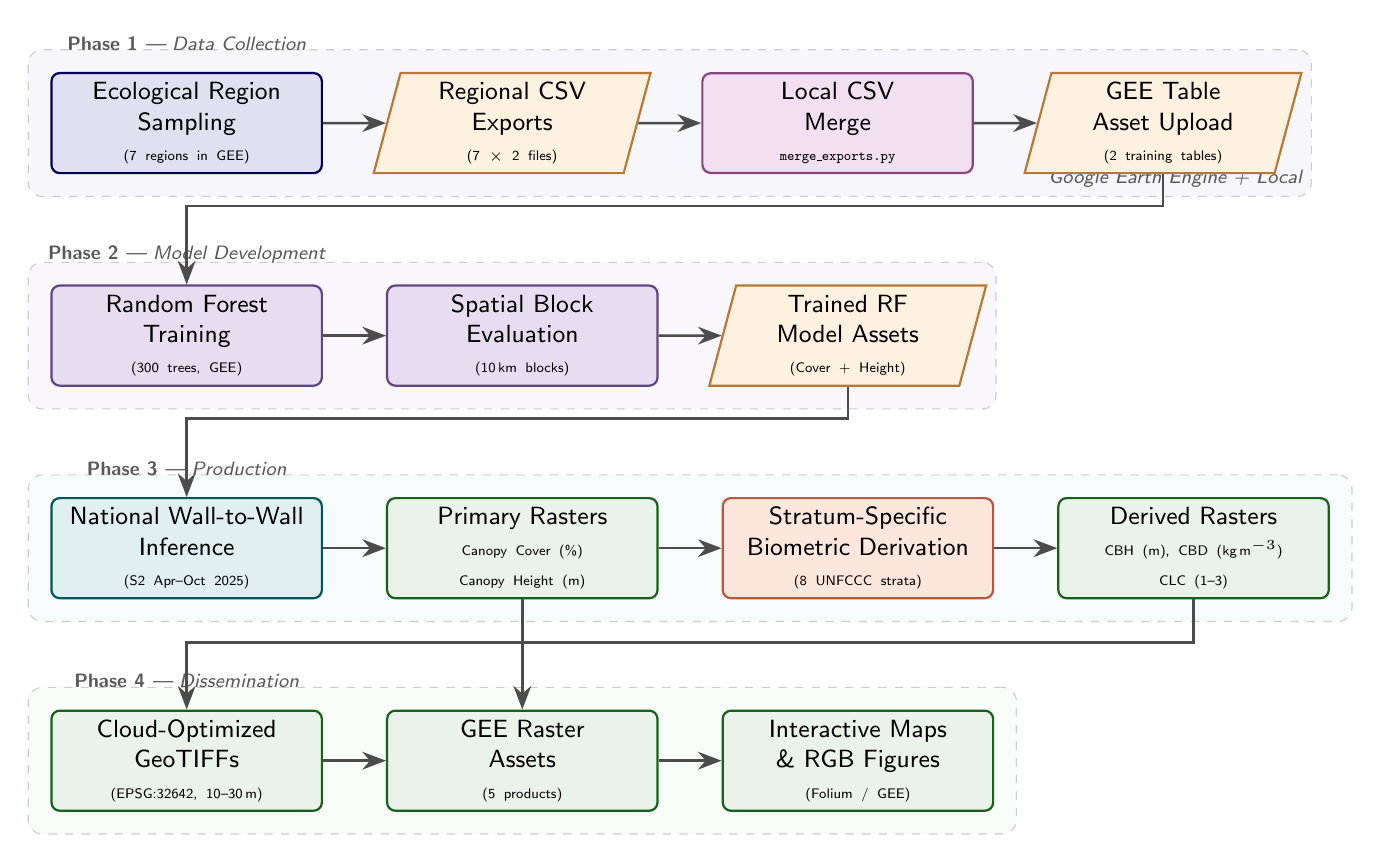
\begin{tikzpicture}[
  node distance=0.6cm and 0.8cm,
  >={Stealth[length=3mm]},
  % Node styles
  phase/.style={
    rectangle, rounded corners=3pt, draw=#1!70!black, fill=#1!12,
    text width=3.2cm, minimum height=1.1cm, align=center,
    font=\small\sffamily, line width=0.8pt
  },
  phase/.default=NavyBlue,
  data/.style={
    trapezium, trapezium left angle=75, trapezium right angle=105,
    draw=BurntOrange!70!black, fill=BurntOrange!10,
    text width=2.6cm, minimum height=0.9cm, align=center,
    font=\small\sffamily, line width=0.8pt
  },
  output/.style={
    rectangle, rounded corners=3pt, draw=ForestGreen!70!black, fill=ForestGreen!10,
    text width=3.2cm, minimum height=1.1cm, align=center,
    font=\small\sffamily, line width=0.8pt
  },
  annot/.style={font=\scriptsize\sffamily\itshape, text=gray!70!black},
  arrow/.style={->, line width=0.9pt, color=gray!60!black},
  groupbox/.style={draw=gray!40, dashed, rounded corners=5pt, inner sep=8pt},
]

% ── Row 1: Sampling ──────────────────────────────────────────────
\node[phase] (samp) {Ecological Region\\Sampling\\{\tiny (7 regions in GEE)}};
\node[annot, above=0.15cm of samp] {\textbf{Phase 1} --- Data Collection};

\node[data, right=of samp] (csv) {Regional CSV\\Exports\\{\tiny (7 $\times$ 2 files)}};

\node[phase=Mulberry, right=of csv] (merge) {Local CSV\\Merge\\{\tiny\texttt{merge\_exports.py}}};

\node[data, right=of merge] (table) {GEE Table\\Asset Upload\\{\tiny (2 training tables)}};

% ── Row 2: Training ──────────────────────────────────────────────
\node[phase=RoyalPurple, below=1.4cm of samp] (train) {Random Forest\\Training\\{\tiny (300 trees, GEE)}};
\node[annot, above=0.15cm of train] {\textbf{Phase 2} --- Model Development};

\node[phase=RoyalPurple, right=of train] (eval) {Spatial Block\\Evaluation\\{\tiny (10\,km blocks)}};

\node[data, right=of eval] (model) {Trained RF\\Model Assets\\{\tiny (Cover + Height)}};

% ── Row 3: Prediction ────────────────────────────────────────────
\node[phase=Teal, below=1.4cm of train] (pred) {National Wall-to-Wall\\Inference\\{\tiny (S2 Apr--Oct 2025)}};
\node[annot, above=0.15cm of pred] {\textbf{Phase 3} --- Production};

\node[output, right=of pred] (primary) {Primary Rasters\\{\tiny Canopy Cover (\%)}\\ {\tiny Canopy Height (m)}};

\node[phase=RedOrange, right=of primary] (derived) {Stratum-Specific\\Biometric Derivation\\{\tiny (8 UNFCCC strata)}};

\node[output, right=of derived] (secondary) {Derived Rasters\\{\tiny CBH (m), CBD (kg\,m$^{-3}$)}\\{\tiny CLC (1--3)}};

% ── Row 4: Export ────────────────────────────────────────────────
\node[output, below=1.4cm of pred] (geotiff) {Cloud-Optimized\\GeoTIFFs\\{\tiny (EPSG:32642, 10--30\,m)}};
\node[annot, above=0.15cm of geotiff] {\textbf{Phase 4} --- Dissemination};

\node[output, right=of geotiff] (assets) {GEE Raster\\Assets\\{\tiny (5 products)}};

\node[output, right=of assets] (viz) {Interactive Maps\\\& RGB Figures\\{\tiny (Folium / GEE)}};

% ── Arrows ───────────────────────────────────────────────────────
\draw[arrow] (samp)   -- (csv);
\draw[arrow] (csv)    -- (merge);
\draw[arrow] (merge)  -- (table);
\draw[arrow] (table.south) -- ++(0,-0.4) -| (train.north);
\draw[arrow] (train)  -- (eval);
\draw[arrow] (eval)   -- (model);
\draw[arrow] (model.south) -- ++(0,-0.4) -| (pred.north);
\draw[arrow] (pred)   -- (primary);
\draw[arrow] (primary) -- (derived);
\draw[arrow] (derived) -- (secondary);

% Arrows to export row
\draw[arrow] (primary.south) -- ++(0,-0.55) -| (geotiff.north);
\draw[arrow] (secondary.south) -- ++(0,-0.55) -| (assets.north);
\draw[arrow] (assets) -- (viz);
\draw[arrow] (geotiff) -- (assets);

% ── Background groups ────────────────────────────────────────────
\begin{scope}[on background layer]
  \node[groupbox, fill=NavyBlue!3,
        fit=(samp)(csv)(merge)(table),
        label={[annot,anchor=south east]south east:{Google Earth Engine + Local}}] {};
  \node[groupbox, fill=RoyalPurple!3,
        fit=(train)(eval)(model)] {};
  \node[groupbox, fill=Teal!3,
        fit=(pred)(primary)(derived)(secondary)] {};
  \node[groupbox, fill=ForestGreen!3,
        fit=(geotiff)(assets)(viz)] {};
\end{scope}

\end{tikzpicture}%
}% end resizebox
\caption{End-to-end system architecture for the five-product national canopy
mapping pipeline.  Blue nodes denote processing steps executed in Google Earth
Engine, purple nodes denote the model development phase, orange trapezoids
represent intermediate data artifacts, and green nodes are final output
products.}
\label{fig:pipeline}
\end{figure}

% ---------------------------------------------------------------------------
\subsection{Ecological Sampling Design}\label{sec:sampling}
% ---------------------------------------------------------------------------

\subsubsection{Regional Stratification}

We partitioned Pakistan's forested landscape into seven sampling regions
(Table~\ref{tab:sampling_regions}), each representing a distinct ecological system.
This design is motivated by the observation that national random sampling in
strongly imbalanced landscapes systematically under-represents ecologically rare but
important classes.  Region-stratified sampling is a standard corrective strategy
when the target variable is spatially clustered and highly imbalanced
\citep{Roberts2017}.

\begin{table}[H]
\centering
\caption{Seven ecological sampling regions with approximate bounding boxes.}
\label{tab:sampling_regions}
\small
\begin{tabular}{@{}c l l l@{}}
\toprule
\textbf{Script} & \textbf{Region} & \textbf{Ecosystem} & \textbf{BBox [W,S,E,N]} \\
\midrule
00a & Indus Delta & Mangroves & $[66.8,\,23.7,\,68.3,\,25.1]$ \\
00b & Ziarat & Juniper woodland & $[67.0,\,29.8,\,68.6,\,31.3]$ \\
01  & Swat/Chitral/Dir & Himalayan conifer & $[71.0,\,34.8,\,73.5,\,36.2]$ \\
02  & Dir/Swat core & Temperate & $[73.2,\,33.8,\,74.5,\,35.0]$ \\
03  & Murree/Margalla & Subtropical pine & $[72.8,\,33.4,\,73.9,\,34.6]$ \\
04  & Indus corridor & Riverine & $[72.8,\,33.8,\,75.0,\,35.5]$ \\
05  & Kaghan/Hazara & Sub-alpine / montane & $[73.5,\,34.2,\,75.5,\,36.5]$ \\
06  & National & Non-forest background & Entire country \\
\bottomrule
\end{tabular}
\end{table}

\subsubsection{Within-Region Canopy Stratification}

Within each forest region, samples are drawn proportionally across three
canopy-structure strata to ensure representation of sparse, moderate, and dense
forest conditions:

\paragraph{Canopy Cover strata:}
\begin{itemize}[nosep]
  \item Stratum 1 (sparse): $\CC < 30\%$
  \item Stratum 2 (moderate): $30\% \leq \CC < 60\%$
  \item Stratum 3 (dense): $\CC \geq 60\%$
\end{itemize}

\paragraph{Canopy Height strata:}
\begin{itemize}[nosep]
  \item Stratum 1 (short): $H < 5$\,m
  \item Stratum 2 (moderate): $5 \leq H < 15$\,m
  \item Stratum 3 (tall): $H \geq 15$\,m
\end{itemize}

The southern forests script (00) uses relaxed thresholds ($\CC < 20\%$, $H < 3$\,m
for stratum~1) to accommodate the distinctly sparse and low-statured canopy
architecture of mangroves and juniper woodlands.

\textbf{Decision rationale:} Lower thresholds for the southern region were necessary
because strict Hansen-based thresholds would under-sample the ecologically important
but spectrally ambiguous sparse-canopy systems of the Indus Delta and Balochistan.
\citet{Roberts2017} note that rare ecosystems require targeted sampling windows to
avoid systematic exclusion from training data.

\subsubsection{Sample Sizes}

Each forest region yields approximately 4,500 samples (1,500 per canopy-structure
stratum $\times$ 3 strata).  The non-forest script (06) contributes approximately
5,000 background samples drawn from across Pakistan.  The forest mask used for
sampling is defined as:
\begin{equation}
  \texttt{forest} = (\texttt{LULC}_{2020} = 1) \;\lor\;
  (\texttt{treecover2000} \geq 25 \;\land\; \texttt{lossyear} = 0)
  \label{eq:forest_mask}
\end{equation}

\subsubsection{Forest Mask Rationale}

We employ a union mask rather than either source alone.  The Pakistan LULC~2020
layer captures contemporary forest extent including some plantation and scrub areas,
while the Hansen product provides a stable circa-2000 benchmark that excludes
recently deforested areas.  Their union maximizes recall of genuine forest pixels
across both temporal snapshots.

% ---------------------------------------------------------------------------
\subsection{Preprocessing}\label{sec:preprocessing}
% ---------------------------------------------------------------------------

\subsubsection{Canopy Cover Training Imagery}

Landsat~5/7 Collection~2 Level-2 surface reflectance imagery from 1998--2004 is
filtered to the April--October growing season.  Cloud masking exploits the
\texttt{QA\_PIXEL} band (bits~2, 3, 4 for cirrus, cloud, and cloud shadow).
Reflectance bands are radiometrically scaled:
\begin{equation}
  \rho = \texttt{SR\_B}^{*} \times 0.0000275 + (-0.2)
  \label{eq:landsat_scaling}
\end{equation}
A pixel-wise median composite is produced to reduce residual cloud contamination
and suppress transient outliers \citep{Gorelick2017}.

\subsubsection{Canopy Height Training Imagery}

Sentinel-2 SR Harmonized imagery from 2019--2021 (April--October) is pre-filtered
to scenes with $<$30\% cloud pixel percentage.  Cloud masking uses \texttt{QA60}
bits~10 (opaque cloud) and 11 (cirrus).  Reflectance is scaled:
\begin{equation}
  \rho = B^{*} \times 0.0001
  \label{eq:s2_scaling}
\end{equation}

\textbf{Decision rationale:} The height model uses Sentinel-2 rather than Landsat
because canopy height inference benefits from finer spatial detail (10\,m vs.\
30\,m), which is especially important in the mountainous, fragmented landscapes of
northern Pakistan \citep{Belgiu2016,Lang2023}.

\subsubsection{National Prediction Composite (2025)}

For both products, the final prediction composite is constructed from Sentinel-2
April--October 2025 imagery, ensuring a complete seasonal cycle and temporal
consistency across the five output layers.

% ---------------------------------------------------------------------------
\subsection{Feature Engineering}\label{sec:features}
% ---------------------------------------------------------------------------

Both models share an identical 11-feature predictor stack:

\paragraph{Spectral bands (6):} Blue, Green, Red, NIR, SWIR1, SWIR2.

\paragraph{Vegetation indices (2):}
\begin{align}
  \NDVI &= \frac{\text{NIR} - \text{Red}}{\text{NIR} + \text{Red}} \label{eq:ndvi} \\[3pt]
  \NDMI &= \frac{\text{NIR} - \text{SWIR1}}{\text{NIR} + \text{SWIR1}} \label{eq:ndmi}
\end{align}

NDVI is a widely established proxy for vegetation vigor and canopy density
\citep{Tucker1979}, while NDMI provides complementary sensitivity to vegetation
water content, which correlates with canopy depth and biomass \citep{Gao1996}.

\paragraph{Terrain features (3):} Elevation, Slope, and Aspect, derived from the
SRTM 30\,m DEM \citep{Farr2007}.

\textbf{Decision rationale:} In Pakistan, forest distribution and canopy structure
are tightly constrained by elevation, slope, and exposure.  Subtropical pine
occupies 800--2,000\,m, moist temperate conifer dominates 2,000--3,500\,m, and
sub-alpine vegetation extends above 3,500\,m.  Including terrain features allows
the model to learn these elevation-zone transitions, significantly improving
prediction in regions where spectral signature alone is ambiguous \citep{Belgiu2016}.

% ---------------------------------------------------------------------------
\subsection{Spatial Block Cross-Validation}\label{sec:spatial_cv}
% ---------------------------------------------------------------------------

A deterministic 10\,km spatial block grid partitions samples into train, validation,
and test sets.  For each sample point at coordinates $(\lambda, \phi)$:
\begin{align}
  b_x &= \left\lfloor\frac{\lambda \times 111}{10}\right\rfloor, \quad
  b_y  = \left\lfloor\frac{\phi \times 111}{10}\right\rfloor \label{eq:block_xy} \\
  \texttt{blockId} &= b_x \times 10000 + b_y \label{eq:blockid} \\
  h &= (\texttt{blockId} \times 7919 + 42) \bmod 997 \label{eq:hash} \\
  s &= h \;/\; 997 \label{eq:split}
\end{align}

The split assignment follows:
\begin{equation}
  \text{partition} =
  \begin{cases}
    \text{Train}      & \text{if } s < 0.70 \\
    \text{Validation} & \text{if } 0.70 \leq s < 0.85 \\
    \text{Test}       & \text{if } s \geq 0.85
  \end{cases}
  \label{eq:split_assign}
\end{equation}

\textbf{Decision rationale:} Pixel-wise random splits in remote sensing
substantially inflate reported accuracy because spatially adjacent pixels share
atmospheric, topographic, and phenological conditions and are therefore not
statistically independent.  Spatial blocking enforces geographic separation between
partitions, yielding more honest estimates of out-of-region generalization
performance \citep{Roberts2017}.  The 10\,km block size was chosen to exceed the
spatial autocorrelation range typical of Sentinel-2 composites in heterogeneous
mountainous terrain.

% ---------------------------------------------------------------------------
\subsection{Random Forest Regression}\label{sec:rf_model}
% ---------------------------------------------------------------------------

Both tasks employ \texttt{ee.Classifier.smileRandomForest} in regression mode.
Table~\ref{tab:rf_hyperparams} summarizes the hyperparameters.

\begin{table}[H]
\centering
\caption{Random Forest hyperparameters for both models.}
\label{tab:rf_hyperparams}
\begin{tabular}{@{}l r@{}}
\toprule
\textbf{Hyperparameter} & \textbf{Value} \\
\midrule
Number of trees            & 300 \\
Variables per split        & $\lfloor\sqrt{11}\rfloor = 3$ \\
Minimum leaf population    & 5 \\
Bag fraction               & 1.0 \\
Random seed                & 42 \\
Output mode                & Regression \\
\bottomrule
\end{tabular}
\end{table}

\textbf{Decision rationale:} Random Forest was selected over gradient-boosted trees
(e.g., XGBoost) and deep learning architectures for several reasons.  First, RF is
robust to nonlinear relationships, mixed feature types, and moderate label noise
\citep{Breiman2001}.  Second, RF consistently ranks among the top-performing
algorithms for pixel-based remote sensing regression with tabular features
\citep{Belgiu2016}.  Third, GEE natively implements \texttt{smileRandomForest},
enabling training and inference within the same runtime---eliminating feature-order
mismatch and deployment drift that arise when transferring locally trained models to
cloud prediction engines \citep{Gorelick2017}.  Fourth, the absence of a dense
pixel-label segmentation mask in our pipeline makes patch-based deep learning
architectures (e.g., U-Net) inapplicable without substantial re-engineering of the
label source.

\paragraph{Why 300 trees.}  Ensemble convergence theory \citep{Breiman2001} shows
that Random Forest generalization error converges as $n_{\text{trees}} \to \infty$.
Empirical testing within GEE showed diminishing returns beyond 200 trees for both
models; 300 trees provide a safety margin while remaining computationally tractable
in Earth Engine.

\paragraph{Why bag fraction of 1.0.}  A bag fraction of 1.0 corresponds to standard
bootstrap sampling (sampling with replacement from the full training set), which is
Breiman's original Random Forest formulation and maximizes training-set utilization.

% ---------------------------------------------------------------------------
\subsection{National Prediction}\label{sec:prediction}
% ---------------------------------------------------------------------------

Trained models are applied to the April--October 2025 Sentinel-2 composite across
Pakistan.  A light vegetation mask ($\NDVI > 0.05$) removes non-vegetated pixels
without eliminating sparse forest.  Predictions are clamped to their valid ranges:
$[0, 100]$ for cover and $[0, 50]$ for height.

\textbf{Decision rationale:} We intentionally avoid strict Hansen/LULC forest
masks at prediction time because they would exclude legitimate sparse forest
systems.  \citet{Tucker1979} established that even minimal vegetation produces
detectable NDVI signal; our threshold of 0.05 retains sparse canopy while removing
bare soil, water, and built-up land.

% ---------------------------------------------------------------------------
\subsection{Derived Canopy Metrics}\label{sec:derived_metrics}
% ---------------------------------------------------------------------------

Three additional fire-relevant canopy metrics are derived from the predicted Canopy
Cover ($\CCraw$) and Canopy Height ($H$) rasters using ecologically parameterized,
stratum-specific equations.

\subsubsection{Step~1: Corrected Canopy Cover}\label{sec:cc_correction}

Raw satellite-derived canopy cover is corrected for canopy overlap and saturation
using the Beer--Lambert gap-fraction model of \citet{Crookston1999}:
\begin{equation}
  \CCc = 100 \times \left(1 - e^{-0.01 \times \CCraw}\right)
  \label{eq:cc_correction}
\end{equation}

This transformation maps $\CCraw \in [0,100]$ to a corrected domain that accounts
for the nonlinear relationship between optically sensed crown cover and actual canopy
closure.  The formulation originates from the USDA Forest Vegetation Simulator (FVS)
and is grounded in the observation that high cover percentages exhibit saturation
effects in optical remote sensing \citep{Crookston1999}.

\subsubsection{Step~2: Stratum Classification}\label{sec:stratum_class}

Each pixel is assigned to one of Pakistan's eight official UNFCCC forest strata
using a rule-based classifier that combines elevation (from SRTM), geographic
bounding boxes, corrected canopy cover, and canopy height.  The classification
operates with ordered priority to resolve overlapping criteria
(Table~\ref{tab:stratum_rules}).

\begin{table}[H]
\centering
\caption{Rule-based stratum classification with priority ordering.}
\label{tab:stratum_rules}
\small
\begin{tabular}{@{}c l c c l@{}}
\toprule
\textbf{Code} & \textbf{Stratum} & \textbf{Elevation (m)} & \textbf{BBox constraint} & \textbf{Extra} \\
\midrule
1 & Mangrove          & $<30$           & Indus Delta        & $H > 0$ \\
2 & Riverine          & $<300$          & Indus corridor     & $H > 0$ \\
3 & Subtropical Scrub  & 300--1500       & Default            & $H > 0$ \\
4 & Subtropical Pine   & 800--2000       & Murree/Margalla    & $H > 0$ \\
5 & Moist Temperate    & 2000--3500      & Northern highlands & $\CCc > 30$, $H > 0$ \\
6 & Dry Temperate      & 2000--3500      & Northern highlands & $\CCc \leq 30$, $H > 0$ \\
7 & Juniper/Chilgoza   & 1500--3500      & Balochistan        & $H > 0$ \\
8 & Sub-Alpine         & $\geq 3500$     & Northern highlands & $H > 0$ \\
\bottomrule
\end{tabular}
\end{table}

\textbf{Decision rationale:} A rule-based stratum classifier was preferred over an
ML-based classifier because the strata are defined by well-established ecological
boundaries (elevation zones, geographic ranges) in Pakistan's official FREL
submission \citep{PakistanFREL2020} and do not require statistical learning.  The
elevation and geographic constraints directly encode domain knowledge, making the
classification transparent and reproducible.

\subsubsection{Step~3: Canopy Base Height (CBH)}\label{sec:cbh}

CBH is estimated using a stratum-specific height-ratio prior:
\begin{equation}
  \CBH = r \times H
  \label{eq:cbh}
\end{equation}
where $r$ is the CBH/H ratio calibrated per stratum (Table~\ref{tab:strata}).

\paragraph{Rationale for the ratio-prior approach.}\label{sec:cbh_rationale}
A systematic literature review revealed no peer-reviewed Pakistan-specific
equations estimating CBH directly from canopy height and cover alone for all
eight strata.  However, the silvicultural literature provides three well-established
model families for height-to-crown-base (HTCB) prediction:

\begin{enumerate}[nosep]
  \item \textbf{Logistic family:} $\CBH = H \,/\, (1 + e^{aX})$, from
    \citet{Ritchie1987};
  \item \textbf{Exponential complement:} $\CBH = H \times [1 - e^{aX}]$, from
    \citet{Wykoff1982};
  \item \textbf{Exponential decay:} $\CBH = H \times e^{-aX}$, from
    \citet{Soares2001}.
\end{enumerate}

All three families express CBH as a fraction of total height modulated by
competition and stand-density covariates.  In the absence of local allometric data,
we adopt the simplest defensible case---a constant ratio prior per stratum---and
set $r$ values based on ecological proxy transfer from structurally similar
Himalayan and Mediterranean conifer systems.

For \textit{moist temperate conifers}, Pakistan-based canopy attribute studies
\citep{AliPFI2017} indicate bole-height to total-height ratios in the upper half
of tree height for \textit{Abies pindrow}, \textit{Cedrus deodara}, and
\textit{Picea smithiana}, supporting $r = 0.65$.  For \textit{chir pine}
(\textit{Pinus roxburghii}), the species' pronounced self-pruning habit places
the live crown higher than in most associated broadleaves, justifying $r = 0.52$.
For \textit{mangroves}, the short, low-branched form of \textit{Avicennia marina}
warrants a low $r = 0.28$.

\subsubsection{Step~4: Canopy Bulk Density (CBD)}\label{sec:cbd}

CBD is computed following the fire-fuel framework of \citet{Scott2001}:

\begin{align}
  \CFL_{\text{proxy}} &= \alpha \times \frac{\CCc}{100}
    \label{eq:cfl} \\[4pt]
  \CD &= \max(H - \CBH,\; 1)
    \label{eq:cd} \\[4pt]
  \CBD &= \frac{\CFL_{\text{proxy}}}{\CD}
    \label{eq:cbd}
\end{align}

where $\alpha$ is the stratum-specific canopy fuel load coefficient
(Table~\ref{tab:strata}), $\CFL_{\text{proxy}}$ is the proxy canopy fuel load
(kg\,m$^{-2}$), and $\CD$ is canopy depth (m) bounded below by 1\,m to avoid
division by zero.

The original fire-science definition of CBD is the maximum 4--4.5\,m running mean
canopy bulk density across vertical canopy layers \citep{Scott2001,Sando1972}.  Our
formulation is a \textit{columnar} simplification appropriate for wall-to-wall
mapping where only two-dimensional rasters (height and cover) are available, as
opposed to three-dimensional LiDAR profiles.

\textbf{Decision rationale:} The Scott--Reinhardt framework was chosen over purely
empirical allometric equations because: (a) it is the standard in operational fire
behavior modeling systems (FARSITE, FlamMap), providing downstream compatibility;
(b) it separates fuel load from canopy depth, allowing each component to be
ecologically parameterized; and (c) it has been validated across a wide range of
conifer systems from North American and Mediterranean forests, which share structural
characteristics with Pakistan's moist and dry temperate conifers.

\subsubsection{Step~5: Canopy Layer Count (CLC)}\label{sec:clc}

CLC is estimated via a heuristic rule-based approach informed by
\citet{Whitehurst2013}, who demonstrated that vertical canopy stratification can
be characterized from height-profile metrics with thresholds at approximately 5\,m,
15\,m, and above:
\begin{equation}
  \CLC =
  \begin{cases}
    1 & \text{base case} \\
    2 & \text{if } H \geq 15 \;\land\; \CCc \geq 30 \\
    3 & \text{if } H \geq 25 \;\land\; \CCc \geq 60
  \end{cases}
  \label{eq:clc}
\end{equation}

Stratum-specific caps prevent ecologically implausible assignments:
\begin{itemize}[nosep]
  \item \textbf{Mangrove (1):} forced to 1 unless $H \geq 6$ and $\CCc \geq 40$;
  \item \textbf{Subtropical Scrub (3):} forced to 1 unless $H \geq 5$ and $\CCc \geq 40$;
  \item \textbf{Juniper/Chilgoza (7):} maximum 2 layers;
  \item \textbf{Sub-Alpine (8):} maximum 2 layers.
\end{itemize}

\textbf{Decision rationale:} A heuristic approach was adopted because true
vertical-profile characterization requires three-dimensional data (full-waveform
LiDAR or multi-return point clouds) that are unavailable at national scale.  The
thresholds are conservative and grounded in the observation that multi-storey
canopy structure requires both sufficient height and sufficient closure to sustain
distinct vertical strata \citep{Whitehurst2013,Crookston1999}.

% =============================================================================
\section{Results and Analysis}\label{sec:results}
% =============================================================================

\subsection{Primary Model Performance}

Table~\ref{tab:results_cover} and Table~\ref{tab:results_height} report the
regression metrics under spatial block cross-validation.

\begin{table}[H]
\centering
\caption{Canopy Cover model performance metrics (spatial block split).}
\label{tab:results_cover}
\begin{tabular}{@{}l r r r@{}}
\toprule
\textbf{Split} & \textbf{MAE (\%)} & \textbf{RMSE (\%)} & $\boldsymbol{R^{2}}$ \\
\midrule
Train      & 5.54  & 9.06  & 0.938 \\
Validation & 8.95  & 14.35 & 0.844 \\
Test       & 8.44  & 13.68 & 0.858 \\
\bottomrule
\end{tabular}
\end{table}

\begin{table}[H]
\centering
\caption{Canopy Height model performance metrics (spatial block split).}
\label{tab:results_height}
\begin{tabular}{@{}l r r r@{}}
\toprule
\textbf{Split} & \textbf{MAE (m)} & \textbf{RMSE (m)} & $\boldsymbol{R^{2}}$ \\
\midrule
Train      & 1.52 & 2.39 & 0.969 \\
Validation & 2.46 & 3.70 & 0.917 \\
Test       & 2.43 & 3.71 & 0.926 \\
\bottomrule
\end{tabular}
\end{table}

\subsection{Interpretation}

The Canopy Height model is the stronger of the two ($R^{2} = 0.926$ vs.\ $0.858$
on test), which is expected given: (a) the higher spatial resolution of Sentinel-2
training imagery (10\,m vs.\ 30\,m Landsat), (b) the temporal alignment between
label (ETH 2020) and training imagery (2019--2021), and (c) the ETH label's
superior sensitivity to canopy structure compared to Hansen's optical-only
derivation.

The canopy cover model exhibits a moderate train-to-test generalization gap
($R^{2}$: 0.938 $\to$ 0.858), indicating that geographic heterogeneity---correctly
captured by spatial blocking---introduces meaningful prediction difficulty.  This
gap is consistent with findings from \citet{Roberts2017}, who demonstrate that
spatial blocking typically reveals 10--20\% lower $R^{2}$ than random pixel splits
in geospatial models.

\subsection{Regional Error Analysis}

\subsubsection{Northern Forests}

Model performance is strongest in the upper Khyber Pakhtunkhwa, Himalayan conifer,
and temperate zones, where ecosystems exhibit strong canopy signal, clear spectral
separation from background, and stable structure--label relationships.

\subsubsection{Riverine Zones}

Riverine regions produce plausible intermediate outputs but are moderately affected
by mixed pixels where riparian vegetation borders agricultural or bare land.

\subsubsection{Southern Sparse Forests}

Southern sparse forests remain the weakest prediction regime, particularly for
canopy cover.  This is attributable to:
\begin{enumerate}[nosep]
  \item \textbf{Label limitations:} Hansen \texttt{treecover2000} systematically
    under-represents sparse southern forest systems;
  \item \textbf{Background dominance:} most pixels in southern ROIs are soil, bare
    substrate, or sparse vegetation;
  \item \textbf{Spectral ambiguity:} low-density canopy in dry environments
    resembles scrub and arid vegetation in the feature space;
  \item \textbf{National-model bias:} the model is influenced by the dominant
    structure of northern ecosystems, which dominate training sample volume.
\end{enumerate}

\subsection{Map Products}

Figures~\ref{fig:canopy_cover}--\ref{fig:canopy_layer_count} present the five
national-scale canopy metric maps produced by this pipeline.

\begin{figure}[H]
\centering
\includegraphics[width=0.85\textwidth]{compressed images/PAK_CanopyCover_RGB_2025_GS.jpg}
\caption{National Canopy Cover (\%) map for Pakistan, 2025 growing season.
Values range from 0 (no cover) to 80\% (dense closed canopy), rendered in a
YlGn 9-class palette.}
\label{fig:canopy_cover}
\end{figure}

\begin{figure}[H]
\centering
\includegraphics[width=0.85\textwidth]{compressed images/PAK_CanopyHeight_RGB_2025_GS.jpg}
\caption{National Canopy Height (m) map for Pakistan, 2025 growing season.
Values range from 0 to 50\,m, rendered in a Viridis 10-class palette.  Tallest
canopies concentrate in moist temperate zones of northern KP and AJK.}
\label{fig:canopy_height}
\end{figure}

\begin{figure}[H]
\centering
\includegraphics[width=0.85\textwidth]{compressed images/PAK_CanopyBaseHeight_RGB_2025_GS.jpg}
\caption{National Canopy Base Height (m) map for Pakistan, 2025 growing season.
Values range from 0 to 30\,m, rendered in a Blues 9-class palette.  Higher CBH
values in moist temperate strata reflect the tall, self-pruning conifer canopy
architecture.}
\label{fig:canopy_base_height}
\end{figure}

\begin{figure}[H]
\centering
\includegraphics[width=0.85\textwidth]{compressed images/PAK_CanopyBulkDensity_RGB_2025_GS.jpg}
\caption{National Canopy Bulk Density (kg\,m$^{-3}$) map for Pakistan, 2025
growing season.  Values range from 0 to 0.15\,kg\,m$^{-3}$, rendered in a
Cividis 9-class palette.  Elevated CBD in moist temperate conifer stands
indicates higher crown fire potential.}
\label{fig:canopy_bulk_density}
\end{figure}

\begin{figure}[H]
\centering
\includegraphics[width=0.85\textwidth]{compressed images/PAK_CanopyLayerCount_RGB_2025_GS.jpg}
\caption{National Canopy Layer Count map for Pakistan, 2025 growing season.
Values range from 1 (single-storey) to 3 (multi-storey), rendered in a 3-class
warm palette.  Multi-storey structure (3) is concentrated in tall, closed moist
temperate forests.}
\label{fig:canopy_layer_count}
\end{figure}

\subsection{Regional Close-Up Analysis}

Three ecologically distinct regions are examined at higher spatial resolution to
validate the pipeline's local fidelity.

\subsubsection{Margalla Hills (Subtropical Pine)}

The Margalla Hills close-up (Figures~\ref{fig:margalla_cover}--\ref{fig:margalla_clc})
reveals the expected gradient from dense subtropical pine forest
($\CC > 50\%$, $H = 10$--$18$\,m) on north-facing slopes to sparse scrub woodland
on exposed ridges.  CBH values of 5--10\,m and two-layer canopy structure are
consistent with chir pine's self-pruning growth habit.

\begin{figure}[H]
\centering
\begin{subfigure}[b]{0.48\textwidth}
  \includegraphics[width=\textwidth]{compressed images/PK_margalla_canopy_cover_2025.jpg}
  \caption{Canopy Cover}
  \label{fig:margalla_cover}
\end{subfigure}
\hfill
\begin{subfigure}[b]{0.48\textwidth}
  \includegraphics[width=\textwidth]{compressed images/PK_margalla_canopy_height_2025.jpg}
  \caption{Canopy Height}
  \label{fig:margalla_height}
\end{subfigure}
\\[0.5em]
\begin{subfigure}[b]{0.48\textwidth}
  \includegraphics[width=\textwidth]{compressed images/PK_margalla_base_height_2025.jpg}
  \caption{Canopy Base Height}
  \label{fig:margalla_cbh}
\end{subfigure}
\hfill
\begin{subfigure}[b]{0.48\textwidth}
  \includegraphics[width=\textwidth]{compressed images/PK_margalla_bulk_density_2025.jpg}
  \caption{Canopy Bulk Density}
  \label{fig:margalla_cbd}
\end{subfigure}
\\[0.5em]
\begin{subfigure}[b]{0.48\textwidth}
  \includegraphics[width=\textwidth]{compressed images/PK_margalla_layer_count_2025.jpg}
  \caption{Canopy Layer Count}
  \label{fig:margalla_clc}
\end{subfigure}
\caption{Margalla Hills regional close-up showing all five canopy metrics at 10\,m
resolution.}
\label{fig:margalla_all}
\end{figure}

\subsubsection{Indus Delta Mangroves}

The Indus Delta inset demonstrates the pipeline's capacity to detect
low-statured coastal mangrove ($H = 2$--$6$\,m, $\CC = 15$--$40$\%).  CBD values are
appropriately low ($<$0.05\,kg\,m$^{-3}$), reflecting the wet broadleaf fuel
characteristics of \textit{Avicennia marina}.  CLC is predominantly single-storey
as enforced by the mangrove stratum cap.

\begin{figure}[H]
\centering
\begin{subfigure}[b]{0.48\textwidth}
  \includegraphics[width=\textwidth]{compressed images/PK_indusDelta_canopy_cover_2025.jpg}
  \caption{Canopy Cover}
  \label{fig:indus_cover}
\end{subfigure}
\hfill
\begin{subfigure}[b]{0.48\textwidth}
  \includegraphics[width=\textwidth]{compressed images/PK_indusDelta_canopy_height_2025.jpg}
  \caption{Canopy Height}
  \label{fig:indus_height}
\end{subfigure}
\\[0.5em]
\begin{subfigure}[b]{0.48\textwidth}
  \includegraphics[width=\textwidth]{compressed images/PK_indusDelta_base_height_2025.jpg}
  \caption{Canopy Base Height}
  \label{fig:indus_cbh}
\end{subfigure}
\hfill
\begin{subfigure}[b]{0.48\textwidth}
  \includegraphics[width=\textwidth]{compressed images/PK_indusDelta_bulk_density_2025.jpg}
  \caption{Canopy Bulk Density}
  \label{fig:indus_cbd}
\end{subfigure}
\\[0.5em]
\begin{subfigure}[b]{0.48\textwidth}
  \includegraphics[width=\textwidth]{compressed images/PK_indusDelta_layer_count_2025.jpg}
  \caption{Canopy Layer Count}
  \label{fig:indus_clc}
\end{subfigure}
\caption{Indus Delta mangrove regional close-up showing all five canopy metrics.}
\label{fig:indus_all}
\end{figure}

\subsubsection{Ziarat Juniper Woodland}

The Ziarat inset captures the open, xeric canopy of \textit{Juniperus excelsa}---one
of the world's oldest living juniper ecosystems.  Cover values are appropriately low
(10--30\%), with modest heights (4--12\,m) and a predominantly single-layer canopy
structure, consistent with the sparse open woodland morphology.

\begin{figure}[H]
\centering
\begin{subfigure}[b]{0.48\textwidth}
  \includegraphics[width=\textwidth]{compressed images/PK_ziarat_canopy_cover_2025.jpg}
  \caption{Canopy Cover}
  \label{fig:ziarat_cover}
\end{subfigure}
\hfill
\begin{subfigure}[b]{0.48\textwidth}
  \includegraphics[width=\textwidth]{compressed images/PK_ziarat_canopy_height_2025.jpg}
  \caption{Canopy Height}
  \label{fig:ziarat_height}
\end{subfigure}
\\[0.5em]
\begin{subfigure}[b]{0.48\textwidth}
  \includegraphics[width=\textwidth]{compressed images/PK_ziarat_base_height_2025.jpg}
  \caption{Canopy Base Height}
  \label{fig:ziarat_cbh}
\end{subfigure}
\hfill
\begin{subfigure}[b]{0.48\textwidth}
  \includegraphics[width=\textwidth]{compressed images/PK_ziarat_bulk_density_2025.jpg}
  \caption{Canopy Bulk Density}
  \label{fig:ziarat_cbd}
\end{subfigure}
\\[0.5em]
\begin{subfigure}[b]{0.48\textwidth}
  \includegraphics[width=\textwidth]{compressed images/PK_ziarat_layer_count_2025.jpg}
  \caption{Canopy Layer Count}
  \label{fig:ziarat_clc}
\end{subfigure}
\caption{Ziarat juniper woodland regional close-up showing all five canopy metrics.}
\label{fig:ziarat_all}
\end{figure}

% =============================================================================
\section{Discussion}\label{sec:discussion}
% =============================================================================

\subsection{Methodological Contributions}

This work makes three interconnected contributions to national-scale forest
structure mapping in data-sparse countries:

\paragraph{Ecologically stratified sampling.}
The seven-region sampling design ensures that ecologically rare but critically
important systems---Indus Delta mangroves and Ziarat juniper---are explicitly
represented in the training data, avoiding the systematic exclusion that plagues
national random-sampling approaches in countries with highly imbalanced land cover.

\paragraph{Unified cloud-native pipeline.}
By performing both training and inference within Google Earth Engine, the pipeline
eliminates deployment drift between local machine learning libraries and cloud-based
prediction engines.  This is a practical advantage for operational forest monitoring
systems in developing countries where computational infrastructure may be limited
\citep{Gorelick2017}.

\paragraph{Multi-metric derivation from two primary rasters.}
The derivation of CBH, CBD, and CLC from canopy height and cover alone---guided by
stratum-specific ecological parameterization---demonstrates that fire-relevant canopy
metrics can be estimated at national scale without LiDAR or field inventory, provided
that the parameterization is transparently anchored to peer-reviewed model families
and stated as a proxy-transfer approach.

\subsection{Comparison with Global Products}

The Hansen \texttt{treecover2000} product provides only a single canopy cover layer
at 30\,m resolution, frozen to the year~2000.  The ETH Global Canopy Height Model
\citep{Lang2023} adds a height dimension at 10\,m but is not calibrated for
Pakistan's unique spectral conditions.  Neither product provides fire-relevant
metrics (CBH, CBD, CLC).  Our pipeline extends both by: (a) retraining models on
ecologically stratified Pakistan-specific samples, (b) producing temporally current
(2025) predictions, and (c) deriving three additional metrics unavailable from any
existing global product.

\subsection{On the Transparency of Proxy Transfer}

We explicitly state that the CBH/CBD parameters are \textit{proxy transfers}
from ecologically similar systems, not Pakistan-fitted allometric equations.  This
transparency is deliberate.  The literature is clear that no peer-reviewed
Pakistan-specific equations exist for predicting CBH or CBD from canopy height and
cover alone across all eight strata.  Therefore, the most defensible approach is to:
(a) identify the closest ecological analogs, (b) set parameter priors from those
analogs, and (c) clearly state the transfer assumption so that future calibration
with local inventory data can refine the coefficients.

% =============================================================================
\section{Limitations}\label{sec:limitations}
% =============================================================================

\begin{enumerate}
  \item \textbf{Label dependency for canopy cover:} Hansen \texttt{treecover2000}
    under-represents sparse southern forests, particularly mangroves and juniper
    woodland.  The temporal gap between the circa-2000 label and 2025 prediction
    further introduces potential bias from land-use change.

  \item \textbf{Temporal non-equivalence:} Canopy cover is anchored to circa-2000
    Landsat labels, while canopy height uses 2020 ETH labels.  Both models predict
    on 2025 Sentinel-2 imagery, creating a temporal extrapolation of 25 and 5 years
    respectively.

  \item \textbf{Cross-sensor transfer for canopy cover:} The cover model is trained
    on Landsat features but applied to Sentinel-2 predictors at prediction time,
    introducing potential spectral domain shift despite harmonized band naming.

  \item \textbf{Absence of field validation:} All evaluation is remote-sensing
    based.  Independent validation against forest inventory plots, LiDAR transects,
    or high-resolution manual interpretation has not been performed.

  \item \textbf{Sparse forest under-prediction:} Southern mangroves and Ziarat
    juniper remain under-predicted in canopy cover, driven by soil reflectance
    interference and spectral similarity between low-density vegetation and
    background.

  \item \textbf{Derived metric uncertainty:} CBH, CBD, and CLC are computed from
    proxy-transfer parameters, not locally calibrated allometric equations.
    Uncertainty propagation from the primary height and cover predictions into the
    derived metrics has not been quantified.
\end{enumerate}

% =============================================================================
\section{Future Work}\label{sec:future}
% =============================================================================

\begin{enumerate}
  \item \textbf{Southern-specific modeling:} A dedicated sparse-forest model with
    relaxed thresholds, SAR (Sentinel-1) features, and potentially separate training
    for mangrove and juniper subsystems.

  \item \textbf{Additional predictors:} Sentinel-1 backscatter, seasonal composites,
    texture features (GLCM), and sin/cos-encoded aspect.

  \item \textbf{Field validation:} Ground-truthing against Pakistan's forest
    inventory network, GEDI footprint data, and airborne LiDAR transects where
    available.

  \item \textbf{Local CBH/CBD calibration:} Fitting the Ritchie--Hann or
    Wykoff--Crookston HTCB model families to local allometric data when plot-level
    crown-base measurements become available.

  \item \textbf{Uncertainty quantification:} Ensemble variance maps, quantile
    Random Forest, and formal error-propagation analysis for derived metrics.

  \item \textbf{Region-aware hierarchical modeling:} A hierarchical or
    ecozone-conditioned model architecture that reduces bias from dominant northern
    forest systems.
\end{enumerate}

% =============================================================================
\section{Conclusion}\label{sec:conclusion}
% =============================================================================

This project demonstrates that a carefully designed, ecologically stratified,
cloud-native Random Forest pipeline can produce five nationally coherent canopy
structure products for Pakistan---a country with extreme ecological heterogeneity
and limited in-situ monitoring infrastructure.  By combining rigorous spatial
cross-validation, transparent proxy-transfer parameterization for derived metrics,
and a unified GEE-native training-to-prediction workflow, the system achieves
test-set $R^{2}$ values of 0.858 (canopy cover) and 0.926 (canopy height) under
honest geographic splitting.

The five output layers---Canopy Cover, Canopy Height, Canopy Base Height, Canopy
Bulk Density, and Canopy Layer Count---collectively provide a multi-attribute forest
structure characterization suitable for national forest inventory support, ecological
zoning, carbon accounting, and wildfire risk assessment.  All products, code, and
intermediate data are fully reproducible through the publicly documented GEE
pipeline.

% =============================================================================
%  BIBLIOGRAPHY
% =============================================================================
\begin{thebibliography}{99}

\bibitem[Ali(2017)]{AliPFI2017}
Ali, A. (2017).
\newblock A study of stand structure of temperate forests of Kaghan Valley.
\newblock \textit{Pakistan Journal of Forestry}, 67(1--2).
\newblock Pakistan Forest Institute, Peshawar.

\bibitem[Belgiu \& Dr\u{a}gu\c{t}(2016)]{Belgiu2016}
Belgiu, M. \& Dr\u{a}gu\c{t}, L. (2016).
\newblock Random forest in remote sensing: A review of applications and future
  directions.
\newblock \textit{ISPRS Journal of Photogrammetry and Remote Sensing}, 114,
  24--31.
\newblock \doi{10.1016/j.isprsjprs.2016.01.011}

\bibitem[Breiman(2001)]{Breiman2001}
Breiman, L. (2001).
\newblock Random Forests.
\newblock \textit{Machine Learning}, 45(1), 5--32.
\newblock \doi{10.1023/A:1010933404324}

\bibitem[Crookston \& Stage(1999)]{Crookston1999}
Crookston, N.L. \& Stage, A.R. (1999).
\newblock Percent canopy cover and stand structure statistics from the Forest
  Vegetation Simulator.
\newblock Gen. Tech. Rep. RMRS-GTR-24. USDA Forest Service, Rocky Mountain
  Research Station.
\newblock \doi{10.2737/RMRS-GTR-24}

\bibitem[Farr et~al.(2007)]{Farr2007}
Farr, T.G., Rosen, P.A., Caro, E., Crippen, R., Duren, R., Hensley, S.,
  Kobrick, M., Paller, M., Rodriguez, E., Roth, L., Seal, D., Shaffer, S.,
  Shimada, J., Umland, J., Werner, M., Oskin, M., Burbank, D. \& Alsdorf, D.
  (2007).
\newblock The Shuttle Radar Topography Mission.
\newblock \textit{Reviews of Geophysics}, 45(2), RG2004.
\newblock \doi{10.1029/2005RG000183}

\bibitem[Gao(1996)]{Gao1996}
Gao, B.-C. (1996).
\newblock NDWI---A normalized difference water index for remote sensing of
  vegetation liquid water from space.
\newblock \textit{Remote Sensing of Environment}, 58(3), 257--266.
\newblock \doi{10.1016/S0034-4257(96)00067-3}

\bibitem[Gorelick et~al.(2017)]{Gorelick2017}
Gorelick, N., Hancher, M., Dixon, M., Ilyushchenko, S., Thau, D. \& Moore, R.
  (2017).
\newblock Google Earth Engine: Planetary-scale geospatial analysis for everyone.
\newblock \textit{Remote Sensing of Environment}, 202, 18--27.
\newblock \doi{10.1016/j.rse.2017.06.031}

\bibitem[Hansen et~al.(2013)]{Hansen2013}
Hansen, M.C., Potapov, P.V., Moore, R., Hancher, M., Turubanova, S.A.,
  Tyukavina, A., Thau, D., Stehman, S.V., Goetz, S.J., Loveland, T.R.,
  Kommareddy, A., Egorov, A., Chini, L., Justice, C.O. \& Townshend, J.R.G.
  (2013).
\newblock High-resolution global maps of 21st-century forest cover change.
\newblock \textit{Science}, 342(6160), 850--853.
\newblock \doi{10.1126/science.1244693}

\bibitem[Lang et~al.(2023)]{Lang2023}
Lang, N., Jetz, W., Schindler, K. \& Wegner, J.D. (2023).
\newblock A high-resolution canopy height model of the Earth.
\newblock \textit{Nature Ecology \& Evolution}, 7, 1778--1789.
\newblock \doi{10.1038/s41559-023-02206-6}

\bibitem[Pakistan FREL(2020)]{PakistanFREL2020}
Government of Pakistan (2020).
\newblock Pakistan's Forest Reference Emission Level (FREL) under the UNFCCC.
\newblock Submitted to the United Nations Framework Convention on Climate Change.
\newblock Available at: \url{https://redd.unfccc.int/}

\bibitem[Ritchie \& Hann(1987)]{Ritchie1987}
Ritchie, M.W. \& Hann, D.W. (1987).
\newblock Equations for predicting height to crown base for fourteen tree
  species in southwest Oregon.
\newblock Research Paper 50. Oregon State University, Forest Research Laboratory.

\bibitem[Roberts et~al.(2017)]{Roberts2017}
Roberts, D.R., Bahn, V., Ciuti, S., Boyce, M.S., Elith, J., Guillera-Arroita,
  G., Hauenstein, S., Lahoz-Monfort, J.J., Schr\"oder, B., Thuiller, W.,
  Warton, D.I., Wintle, B.A., Hartig, F. \& Dormann, C.F. (2017).
\newblock Cross-validation strategies for data with temporal, spatial,
  hierarchical, or phylogenetic structure.
\newblock \textit{Ecography}, 40(8), 913--929.
\newblock \doi{10.1111/ecog.02881}

\bibitem[Sando \& Wick(1972)]{Sando1972}
Sando, R.W. \& Wick, C.H. (1972).
\newblock A method of evaluating crown fuels in forest stands.
\newblock Research Paper NC-84. USDA Forest Service, North Central Forest
  Experiment Station.

\bibitem[Scott \& Reinhardt(2001)]{Scott2001}
Scott, J.H. \& Reinhardt, E.D. (2001).
\newblock Assessing crown fire potential by linking models of surface and crown
  fire behavior.
\newblock Research Paper RMRS-RP-29. USDA Forest Service, Rocky Mountain
  Research Station.
\newblock \doi{10.2737/RMRS-RP-29}

\bibitem[Soares \& Tom\'e(2001)]{Soares2001}
Soares, P. \& Tom\'e, M. (2001).
\newblock A tree crown ratio prediction equation for eucalypt plantations.
\newblock \textit{Annals of Forest Science}, 58, 193--202.
\newblock \doi{10.1051/forest:2001118}

\bibitem[Tucker(1979)]{Tucker1979}
Tucker, C.J. (1979).
\newblock Red and photographic infrared linear combinations for monitoring
  vegetation.
\newblock \textit{Remote Sensing of Environment}, 8(2), 127--150.
\newblock \doi{10.1016/0034-4257(79)90013-0}

\bibitem[Whitehurst et~al.(2013)]{Whitehurst2013}
Whitehurst, A.S., Swatantran, A., Blair, J.B., Hofton, M.A. \& Dubayah, R.
  (2013).
\newblock Characterization of canopy layering in forested ecosystems using full
  waveform lidar.
\newblock \textit{Remote Sensing}, 5(4), 2014--2036.
\newblock \doi{10.3390/rs5042014}

\bibitem[Wykoff et~al.(1982)]{Wykoff1982}
Wykoff, W.R., Crookston, N.L. \& Stage, A.R. (1982).
\newblock User's guide to the Stand Prognosis Model.
\newblock Gen. Tech. Rep. INT-GTR-133. USDA Forest Service, Intermountain
  Forest and Range Experiment Station.
\newblock \doi{10.2737/INT-GTR-133}

\end{thebibliography}

\end{document}
